% Appendix section discussing capabilities of the GUI.

\chapter{Schematic Drawing GUI}
\label{app:gui}

One of the aims of this project is making it easy for students to describe the
circuit they have in mind to a computer. To that end, it is important that the
schematic entry tool be intuitive and easy to use. In this section, I will
describe the capabilities and features offered by the schematic entry Graphical
User Interface. Figure \ref{fig:gui} presents the GUI containing a sample
schematic. The figure depicts the four important sections of the GUI: the board,
the palette, the analysis section, and the cursor toggle section.

\begin{figure}
\begin{center}
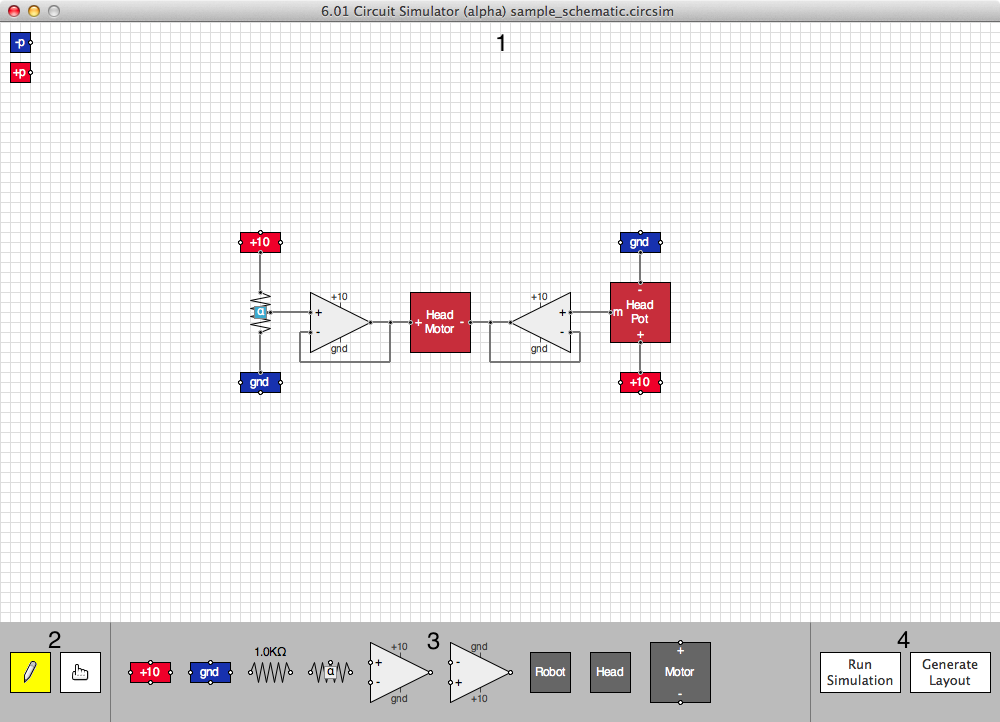
\includegraphics[width=\textwidth]{Images/gui.png}
\caption{Parts of the schematic entry GUI.}
\label{fig:gui}
\end{center}
\end{figure}

\section{Palette}

The palette (item $2$ in Figure \ref{fig:gui}) offers all of the circuit
components that can constitute a 6.01 circuit. Clicking a circuit component on
the palette spawns a new component of the same type on the board right above
the palette. This component can then be used in the circuit construction. The
``Robot" and ``Head" buttons on the palette spawn multiple parts at once
corresponding to the multiple parts contained within each item. The robot
connector contains pins for power and ground as well as for analog input pins
and one analog output pin. The head is composed of a motor, a motor pot, and
two photosensors. Figure \ref{fig:robot_head_parts} demonstrates these last two
circuit components.

\begin{figure}
\begin{center}
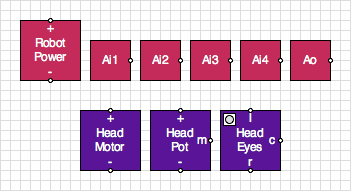
\includegraphics[scale=0.75]{Images/robot_head_parts.png}
\caption{Grouped components: Robot Connector and Head Connector.}
\label{fig:robot_head_parts}
\end{center}
\end{figure}

\section{Board}

The board (item $1$ in Figure \ref{fig:gui}) is where the user can draw circuit
schematics. The user may move a component on the board by clicking the component
and dragging it to the desired place. When dragging, the GUI draws guide lines
that extend to the extents of the board to help the user place the component
at the right place. The user has the option to select and move multiple items at
once.The user may delete a component by clicking on it while
pressing \keystroke{Ctrl}. The user may rotate a component by clicking on it
while pressing \keystroke{Shift}. An important aspect of circuit schematics is
interconnecting components with wires. Each circuit component in the GUI comes
with a few connection points. The user my connect components by drawing wires
that connect these connection points. The user may draw a wire by clicking on a
connection point and dragging. A wire may be drawn to (1) another connection
point, or (2) a wire already on the board, which snaps the new wire onto the
existing wire, or (3) an empty location on the board, which would create a new
connection point. A wire may also be drawn starting from an existing wire,
which creates a new connection point on the existing wire. The GUI allows the
user to drag connection points. To achieve this, the GUI has two possible
states for the cursor, the drawing states and the dragging state (mainly
referring to wires). Item $4$ in Figure \ref{fig:gui} displays the panel that
lets the user toggle between these two states. In the dragging state, the user
can drag connection points just like other circuit components.
When drawing wires,
the GUI attempts to route the wires in a way that is aesthetically pleasing.
That is, the wire is routed so as to avoid crossing wires and, more importantly,
wires crossing components on the board. Note that doing this is not a trivial
task. In fact, this problem is very similar to the layout problem that this
project aims to tackle. The solution to the wiring problem in the GUI also uses
search.

\section{Analysis}

The analysis section of the GUI (item $3$ in Figure \ref{fig:gui}) lets the user
analyze the drawn circuit schematic in two ways.

\subsection{Simulation}

The GUI lets the user simulate the circuit and test whether it behaves as
expected. The simulation infrastructure is ported from CMax, and hence circuits
are simulated exactly as they are simulated by CMax. If there are probes in the
circuit, the simulator presents the voltage difference across the probes as an
output. If there is a motor in the circuit, the simulator presents the motor's
angle and motor's rotational velocity as functions of time. If there are any
pots in the circuit, the user is expected to select a simulation file for each
pot describing how the pot is manipulated as a function of time. Similarly,
if the photosensors are a part of the circuit, the user is expected to select
a simulation file for each photosensor set describing the lamps distance and
angle from the head. These simulations help students (and staff) verify that
they have a correctly functioning circuit before building it.

\subsection{Layout}

The GUI also lets the user generate a layout for the circuit schematic, which is
the main object of this project. Very importantly, the GUI makes it very easy to
relate the schematic with the layout. When the user hovers over a component in
either window, the GUI highlights the corresponding component in the other
window. When the user hovers over a wire in one window, the GUI highlights all
of the wires in both windows that correspond to the same node. Figures
\ref{fig:wire_highlight} and \ref{fig:component_highlight} demonstrate this
feature.

\begin{figure}
\begin{center}
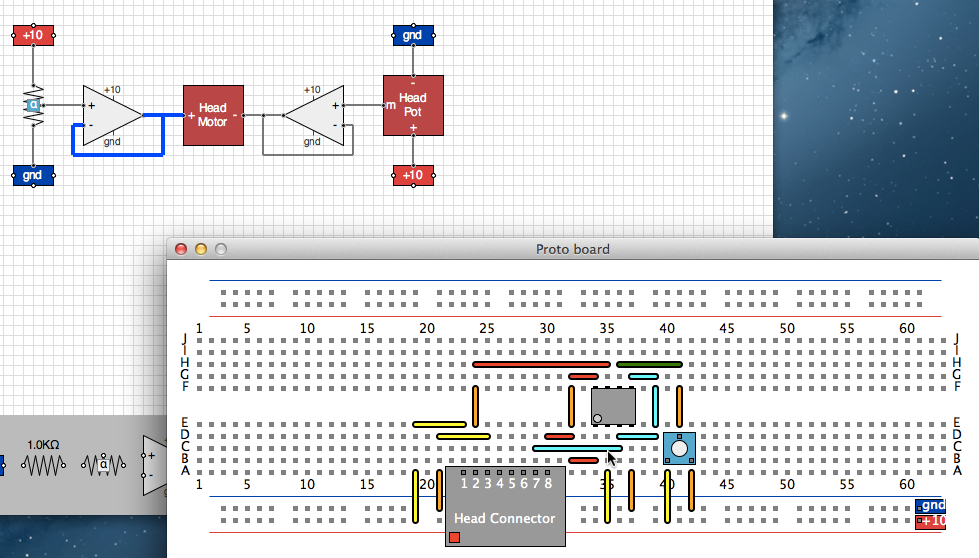
\includegraphics[width=\textwidth]{Images/gui_wire_highlight.png}
\caption{Wire highlighting example.}
\label{fig:wire_highlight}
\end{center}
\end{figure}

\begin{figure}
\begin{center}
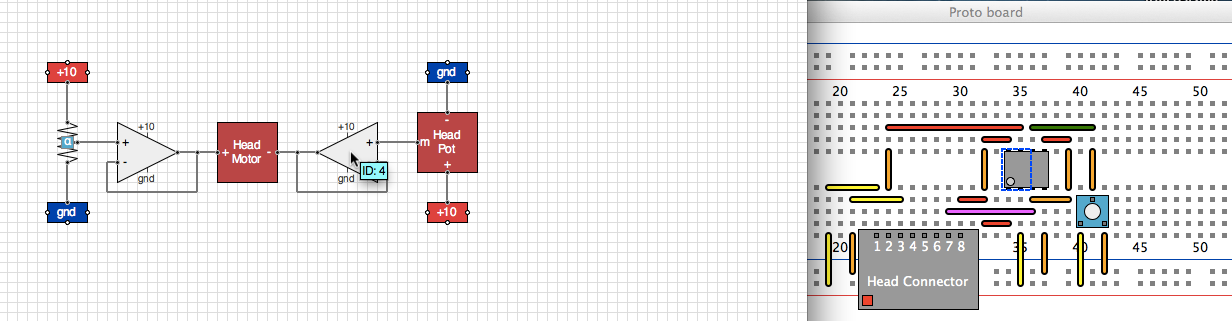
\includegraphics[width=\textwidth]{Images/gui_component_highlight.png}
\caption{Component highlighting example.}
\label{fig:component_highlight}
\end{center}
\end{figure}

\section{Other Features}

Here we discuss several features offered by the GUI that have not been discussed
so far:

\begin{enumerate}
\item The GUI allows the user to save schematics for later viewing or editing.
\item Protoboard layouts can also be saved as CMax files allowing for editing
in CMax.
\item The schematic editing tool allows the user to undo and redo all actions.
\item The GUI has menu items that offer access to some of the features already
discussed. Menu items are added when particular circuit components are selected.
For instance, selecting a pot component results in a new menu item that allows
the user to select a signal file for the pot. The same properties can also be
reached by right-clicking on the components.
\item The GUI changes the cursor appropriately to provide feedback. For instance,
the cursor becomes
a pencil if the user can draw a wire starting at the cursor's current position.
The cursor also changes to indicate when the user is about to rotate or delete
a component. If the tool is busy either running a simulation or generating a
layout, the cursor shows that the tool is busy.
\end{enumerate}

\section{Shortcuts}
Table \ref{tb:shortcuts} presents the shortcuts available in the GUI.

\begin{table}
\begin{center}
\begin{singlespace}
\begin{tabular}{| c | c |}
\hline
Action & Shortcut \\
\hline
\hline
\keystroke{Ctrl} + \keystroke{n} & New file \\
\keystroke{Ctrl} + \keystroke{o} & Open file \\
\keystroke{Ctrl} + \keystroke{s} & Save file \\
\keystroke{Ctrl} + \keystroke{q} & Quit \\
\keystroke{Ctrl} + \keystroke{z} & Undo \\
\keystroke{Ctrl} + \keystroke{y} & Redo \\
\keystroke{Ctrl} + \keystroke{w} & Close simulation windows \\
\keystroke{g} & Generate layout \\
\keystroke{s} & Run simulation \\
\keystroke{Delete} & Delete selected items \\
\keystroke{r} & Rotate selected item \\
\keystroke{d} & Toggle cursor state \\
\keystroke{$\leftarrow$} | \keystroke{h} & Move selected items left \\
\keystroke{$\downarrow$} | \keystroke{j} & Move selected items down \\
\keystroke{$\uparrow$} | \keystroke{k} & Move selected items up \\
\keystroke{$\rightarrow$} | \keystroke{l} & Move selected items right \\
\hline
\end{tabular}
\end{singlespace}
\end{center}
\label{tb:shortcuts}
\caption{Shortcuts.}
\end{table}
